\documentclass[a4paper, 12pt, notitlepage] {article}
\usepackage{color}
\usepackage{verbatim}
\usepackage{graphicx}
\usepackage{enumerate}
\usepackage{turnstile}
\usepackage{centernot}
\renewcommand{\thesubsection}{\alph{subsection}}

\newcommand{\hide}[1]{}
\newcommand{\mscmt}[1]{{\color{blue} \tiny{Srivas: {#1}}}}
\newcommand{\bcmt}[1]{{\color{green} \tiny{Bhishma: {#1}}}}
\newcommand{\hcmt}[1]{{\color{magenta} \tiny{Hitarth: {#1}}}}

\usepackage{amsmath} % American mathematical society package for matrices etc.
\usepackage{amssymb} %American mathematical society symbols
\author{Hitarth \\ Bhishmaraj}
\title{STM Project Proposal}
\date{} %This will make sure that date is not shown by \maketitle command
\begin{document}
\maketitle		


\begin{center}
MSc CS Students, CMI
\end{center}
\begin{center}
October 24, 2019
\end{center}
\newpage

\section{Introduction}

\mscmt{Your motivation for problem should be made as follows:
\begin{enumerate}
\item Solver-aided programming languages and tools, such as Rosette (give ref to PLDI paper) help exploit power of SAT/SMT solvers in designing solutions to domain-specific constraint solving problems.

\item Most of the existing efforts have used SAT solvers have restricted to arithmetic and bit-vector theories

\item In this project we propose to use Rosette-Racket for analysis (verification and synthesis) of  array manipulating programs.

\item Arrays pose a challenge because they are, in general, undecidable and most interesting properties about arrays require quantifier instantiation.

\item We simplify our problem by restricting ourselves to decidable fragments of the arrays theory (give ref of the paper I had uploaded) and the class of programs for analysis.
\end{enumerate}
}

To makes it easier to automate the process of program verification, debugging and synthesis, we usually focus on a (small) set of programming constructs. This makes it possible to automatically encode the program in logical statements such that it's verification etc can be done. \\

For this project we have decided to focus on the simple programs which involve arrays. We will allow the basic operations like accessing and storing in an array.

\section {Problem: Verification, Debugging and Synthesis in straight line array programs}
\mscmt{Please use the following array initializing program as he running example to define and illustrate problem statement.
You can make suitable changes to the program to inject a bug and synthesize the bug fixes.
Your program has hardly any meat in it.\\
Note: Although the example shows a loop, it doesn't mean you are supporting loop verification; implicit assumption here is that the user provides a loop invariantas illustrated in the next picture.
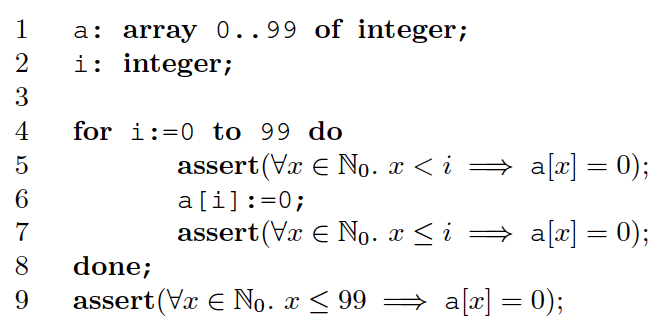
\includegraphics[scale=0.6]{arrayprogex} \\
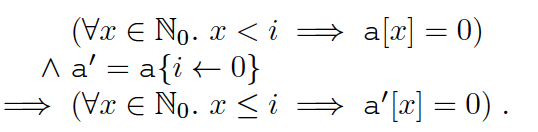
\includegraphics[scale=0.6]{arrayvc} 
}

Consider a simple program as given below:

\begin{verbatim}
/*Program to set a value at a given index 
if it is larger than existing value*/

void update_value(array, index, value){
    if array[index] < value {
        array[index] = value;
    }
}
\end{verbatim}

In this program we are doing a simple operation. We know that the final postcondition would be:  $( a[i] < v \implies a_1[i] == v \land (\forall{j} . j\neq i . a[j] = a_1[j]))    \land (a[i] >= v \implies a_1 = a)$, where $a$ and $a_1$ represent the array before and after the execution of the program respectively.
Given the pre/post conditions, we can ask for the correctness of the program.\\

Usually while writing the programs involving arrays, we might make an error while accessing the arrays. This is exactly what we will be focussing on while synthesizing. We shall assume that the error is only on the accessing operation, and with the help of Rosette we will try to fix that.\\

Our main goals in this project are as follows: \\
\mscmt{Organize the goals as follows:
\begin{enumerate}
\item Methodology: Develop a method of converting the problem of performing the following analysis of a restricted class of array manipulating programs into instances of SMT array logic.
\begin{itemize}
\item Verifying an array manipulating program against its specification given as pre-post conditions and loop invariants (for program with loops).
\item Localizing the location of a bug when verification fails
\item Synthesizing a fix for the bug when there exists a fix within a restricted class of possible fixes
\end{itemize}

\item Implementation of our method within the Rosette-Racket solver-aided programming tool/language framework.\

\item Experiment our implementation on a targeted class of benchmark examples.
\end{enumerate}
}
\begin{enumerate}
	\item To take a program and the pre and post conditions, and verify the correctness of the program using Rosette.
	\item Given two programs, where one is assumed to be correct, verify the correctness of the other suspected program.
	\item If the program is incorrect as per the either the conditions or the second program which is assumed to be correct, find the parts of the program which might be the cause of the error.
	\item If the program is incorrect, then  try to synthesize the correct program by only focussing on the bugs due to {\bf array access operations}.
\end{enumerate}

\section {Approach}
We will firstly define a basic language which only deals with arrays of integers and provides basic functionalities like accessing and storing in an array. Then we will embed this language with basic programming constructs for arrays in Racket/Rosette.\\
\\
Rosette provides us with various tool to verify, debug and synthesize once we write the interpreter in it. We will then explore how we can automate this process and auto fix the bugs related to array accessing.
\\
\\
We will show with examples how we can use this for debugging and synthesis in such programs.\\
\\
We also plan to create a seperate GUI application which can provide an easy to use interface to the user to get these functionalities. 


\section{Expected Results}
We expect to have a system which can take simple array programs and help the user with verification, debugging and synthesis provided they give either pre and post conditions or another program which has the correct behaviour.\\
\\
Almost all the programs use arrays in one way or another, but most of the useful programs involving arrays also have loops. At least for now, our plan is not to indulge with loops. We might consider the loops if we are successful in the first phase of our project. 

\section*{References}

\begin{enumerate}
	\item Rosette Language guide - https://docs.racket-lang.org/rosette-guide/index.html
\end{enumerate}
\end{document}